\section{Summarized results from Study 1}
The initial goal of this study was to derive new analysis frameworks for phylogenetics by representing phylogenetics as something more malleable, for example, a set of features for machine learning. This led to the development of \gls{p2v} (or Phylo2Vec)~\cite{penn2025, scheidwasser2025}, a framework for representing phylogenetic tree topologies as integer vectors. Inspired by Yule processes~\cite{steel2001} and tree counting strategies~\cite{knuth1973, rotem1978, proskurowski1980, rohlf1983}, the core idea of phylo2vec is to describe \emph{how} leaves are iteratively added to an existing tree topology. The construction of phylo2vec builds upon the work of Rohlf~\cite{rohlf1983} and Dinh~\cite{dinh2010}, but differs in its edge labelling strategy and, in the case of Rohlf~\cite{rohlf1983}, in preserving the tree-construction process within the vector representation. Beyond this conceptual shift, our contributions were fourfold: (i) rigorous proofs that the vector representation is bijective with the space of binary rooted trees~\cite{penn2025}, (ii) an extended matrix format to incorporate branch length information, (iii) empirical evidence of its usability for phylogenetic inference, and (iv) robust and open-source software for manipulating phylogenetic trees using this representation~\cite{scheidwasser2025}. % In addition, the simplicity of such a vector format makes it a convenient starting object for phylogenetic tree manipulation, which is showcased in the \texttt{phylo2vec} software package~\cite{scheidwasser2025}. The package also highlights potential avenues for phylo2vec-based phylogenetic inference, including non-traditional optimisation approaches such as (gradient-based \gls{bme} (GradME)~\cite{penn2023}.

% phylo2vec was originally designed with fast sampling, rapid comparison, and efficient compression of phylogenetic trees

The simple constraint of the phylo2vec formulation notably allows for rapid tree sampling, efficient compression, and straightforward comparison of tree topologies. As shown in Fig.~\ref{fig:p2v_sample}, it is notably faster than the widely used tree manipulation libraries \texttt{ete3}~\cite{huerta2016} and  \texttt{ape}~\cite{paradis2019} (Fig.~\ref{fig:p2v_sample}). The distribution of trees generated from phylo2vec sampling is also naturally uniform~\cite{scheidwasser2024}, similar to the proportional-to-distinguishable-arrangements model~\cite{holman2005}.

\begin{figure}[htbp]
    \centering
    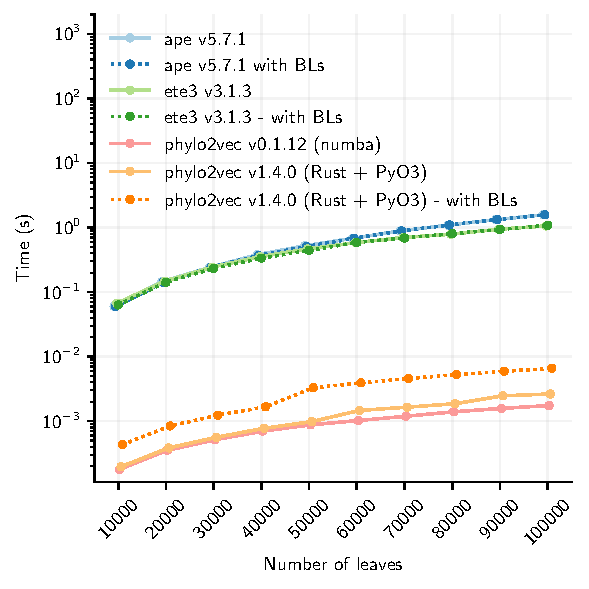
\includegraphics[width=0.5\linewidth]{img/sample_benchmark.pdf}
    \caption{Sampling speed of phylo2vec vectors and matrices. Plain lines denote functions for sampling a single random tree topology. Dotted lines denote functions for sampling a single random tree with random branch lengths (BLs).}
    \label{fig:p2v_sample}
\end{figure}

phylo2vec also allows for fast comparison of binary trees, as illustrated by the deduplication task in Penn \textit{et al.}~\cite{penn2025}. Beyond equality, two tree topologies can be compared using phylo2vec via a simple Hamming distance between their respective vectors, as described in Section~\ref{methods:p2v_properties}. Through random walks in both phylo2vec and tree spaces, we observed that moves in the phylo2vec space \emph{generally} equated with \gls{spr} rearrangements. Linear correlation with the Hamming distance was highest with the \gls{spr} distance (Pearson's $r$: 0.93), and lowest for distance metrics related to \gls{nni} (Fig.~\ref{fig:p2v_dist}). Yet, performing a single \gls{spr} on a tree may still result in a significantly different vector (Fig.~\ref{fig:p2v_metrics_from_moves}), and vice versa for a single vector move (Hamming distance of one) (Fig.~\ref{fig:p2v_metrics_from_v_single}).

\begin{figure}[htbp]
    \centering
    \subfloat[]{%
        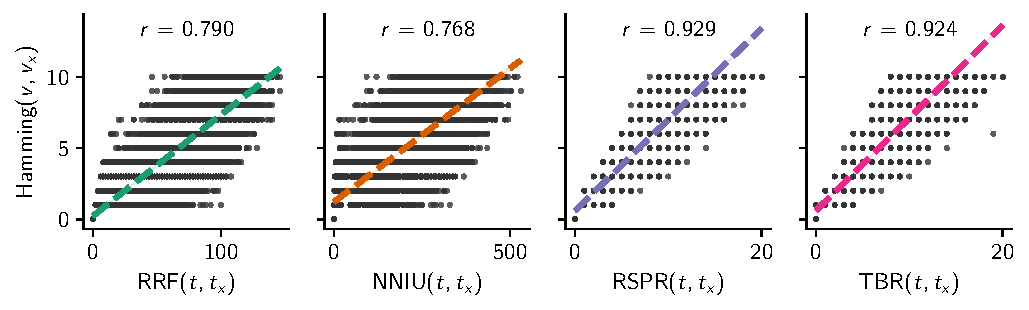
\includegraphics[height=6cm]{img/compare_metrics_from_v.pdf}%
        \label{fig:p2v_metrics_from_v}%
    }
    \subfloat[]{%
        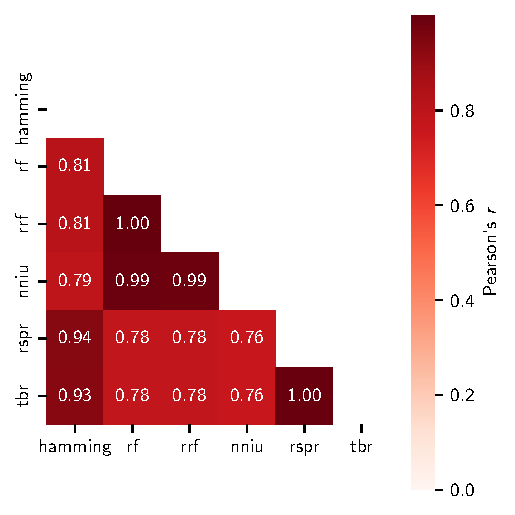
\includegraphics[height=6cm]{img/compare_metrics_from_v_corr.pdf}%
        \label{fig:p2v_metrics_corr}%
    } \\
    \subfloat[\label{fig:p2v_metrics_from_v_single}]{%
        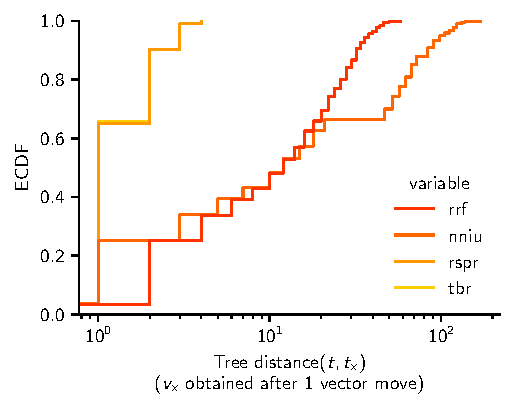
\includegraphics[height=5cm]{img/compare_metrics_from_v_single.pdf}%
        %
    }
    \subfloat[\label{fig:p2v_metrics_from_moves}]{%
        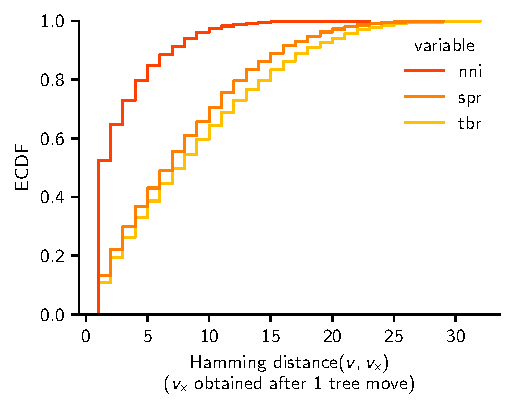
\includegraphics[height=5cm]{img/compare_metrics_from_moves.pdf}%
        %
    }
    \caption{Comparison of phylo2vec topology moves against standard tree rearrangement operations: \gls{nni}, \gls{spr}, \gls{tbr}.}
    \label{fig:p2v_dist}
\end{figure}

Due to its flat vector nature, an immediate property of phylo2vec is its compact format (Fig.~\ref{fig:p2v_compression}). For tree topologies, a phylo2vec vector occupies less memory than the Newick format for trees with 100 leaves or more, and the compression ratio reaches 6x using 16-bit integers (up to $\approx$ 32,000 leaves) and 3x using 32-bit integers (Fig.~\ref{fig:p2v_vs_nwk_int}). For trees with branch lengths, phylo2vec is preferable for large trees (10,000 leaves or more), where the compression ratio reaches 10x for 100,000 leaves (Fig.~\ref{fig:p2v_vs_nwk_float}).

Saving thousands of trees, an operation typically performed in Bayesian phylogenetics involving \gls{mcmc} sampling, can also be optimised using phylo2vec. Although standard file compression (e.g., using \texttt{gzip}) already enables some significant savings, saving 10,000 trees in phylo2vec format can be approximately 5 to 50 times more efficient in terms of file size than a plain-text counterpart (Fig.~\ref{fig:p2v_vs_nwk_int_files},~\ref{fig:p2v_vs_nwk_float_files}).

\begin{figure}[htbp]
    \centering
    % First row
    \subfloat[]{%
        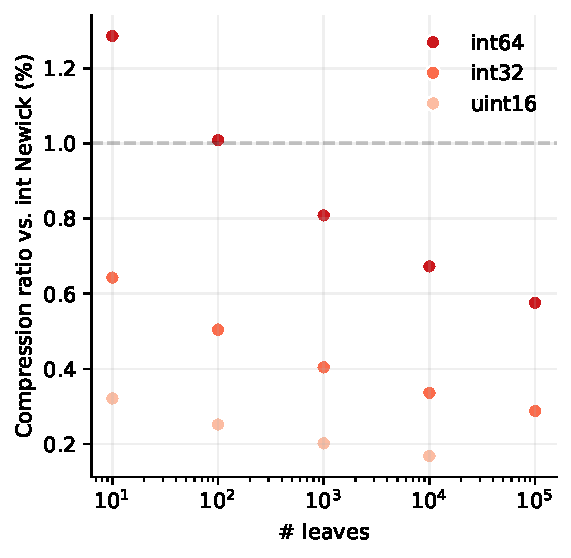
\includegraphics[width=0.4\textwidth]{img/p2v_vs_nwk_int.pdf}%
        \label{fig:p2v_vs_nwk_int}%
    }
    \hspace{0.25cm}
    \subfloat[]{%
        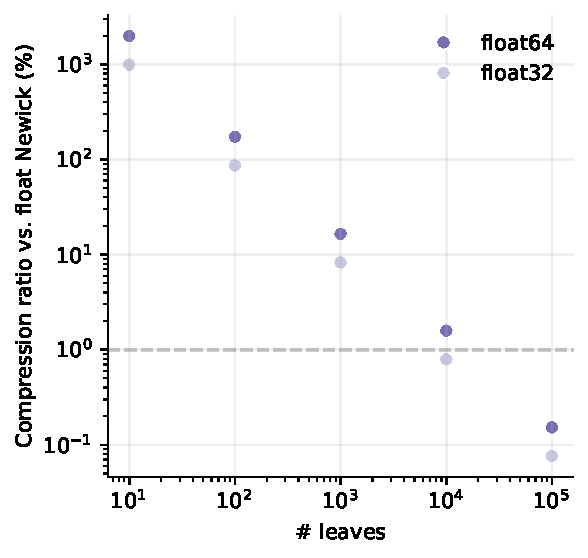
\includegraphics[width=0.4\textwidth]{img/p2v_vs_nwk_float.pdf}%
        \label{fig:p2v_vs_nwk_float}%
    }
    \vspace{0.25cm}
    % Second row
    \subfloat[]{%
        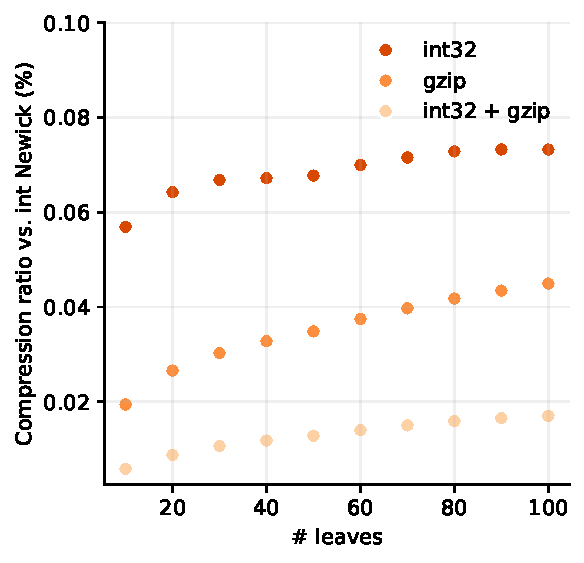
\includegraphics[width=0.4\textwidth]{img/p2v_vs_nwk_int_files.pdf}%
        \label{fig:p2v_vs_nwk_int_files}%
    }
    \hspace{0.25cm}
    \subfloat[]{%
        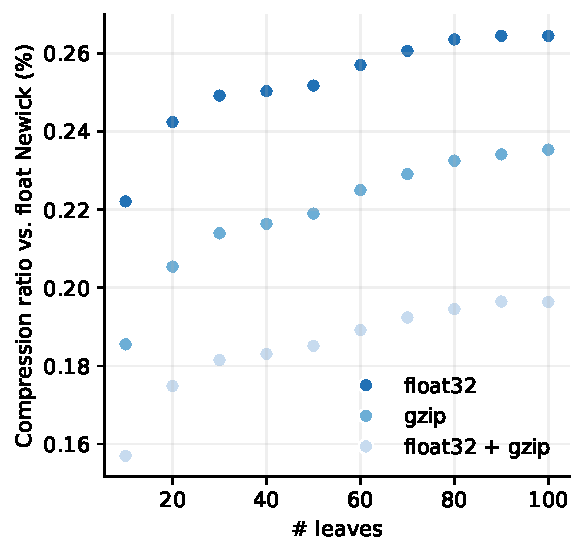
\includegraphics[width=0.4\textwidth]{img/p2v_vs_nwk_float_files.pdf}%
        \label{fig:p2v_vs_nwk_float_files}%
    }
    \caption{Analysing the compactness of the phylo2vec formats against the Newick format. \textsb{(a, b)}: compression ratia of tree topologies (resp. trees with branch lengths) as phylo2vec vectors (resp. as phylo2mat matrices) against their equivalent Newick strings. \textsb{(c, d)}: compression ratia of 10,000 random tree topologies (resp. trees with branch lengths) with coronavirus taxa saved as a plain-text file (often saved with the file extension \texttt{.trees}) vs. a hierarchical data format (HDF) file containing the trees as an array of phylo2vec vectors (resp. array of phylo2mat matrices), and a JSON representation of a mapping of taxon-to-integer labels. }
    \label{fig:p2v_compression}
\end{figure}

As a proof of concept, we demonstrated the feasibility of likelihood-based phylogenetic inference with phylo2vec using a hill-climbing scheme in Section~\ref{methods:p2v_inference} on four simple \glspl{msa}, three of which pertain to viral genes of Zika and Influenza A (Section~\ref{methods:p2v_evaluation}). The hill-climbing technique, which involves performing tree proposals using phylo2vec vectors and leveraging RAxML-NG~\cite{kozlov2019} for branch length and substitution optimisation based on the proposed vector, was generally able to recover a tree with the same likelihood as RAxML-NG used standalone~\cite{penn2025}. Despite starting from random trees, this scheme only required a fraction of tree proposals compared to the space of possible trees~\cite{penn2025}, thereby demonstrating that it can efficiently traverse tree space. However, our approach is more prone to being trapped in local optima due to the pulley principle~\cite{felsenstein2004}, whereby multiple rooted trees can have identical likelihoods when they represent different root placements of the same underlying topology. This creates optimisation challenges that are not typically encountered by most likelihood-based methods, which operate with unrooted trees~\cite{kozlov2019, minh2020}.

Overall, the simplicity of such a vector format makes it a convenient starting object for phylogenetic tree manipulation, as showcased in the \texttt{phylo2vec} software package~\cite{scheidwasser2025}. The package also highlights other potential avenues for phylo2vec-based phylogenetic inference, including scripts to calculate the likelihood of a phylo2mat matrix using BEAGLE~\cite{ayres2019} and non-traditional optimisation approaches such as (gradient-based \gls{bme} (GradME)~\cite{penn2023}).

\clearpage
\section{Summarized results from Study 2}
The overarching goal of this study was to evaluate the informational utility of structure-based phylogenetics to complement our understanding of viral evolution. To this end, we gathered experimental spike glycoprotein structures from the \gls{pdb}~\cite{berman2000, rose2010} of various species of the \textit{Betacoronavirus} genus. We used Foldseek~\cite{vankempen2024} to translate the structures into discrete sequences and MAST~\cite{wong2024} to analyse how recombination shapes the structural evolution of spike proteins.

Mixture modelling showed different classes in spike for RBD/NTD/S2.
Less precise with 3di, but similar pattern.

\clearpage
\section{Summarized results from Study 3}
The last study of this thesis aimed to detect infection in poultry using a deep learning-based framework to analyse animal behaviour from video data. To this end, we designed a pilot study to assess welfare impairments caused by \textit{E. coli} infection in broiler chickens~\cite{scheidwasser2024}. Two groups of 20 broiler chickens, one control group and one group infected with \textit{E. coli}, were monitored during the infection phase through video recordings. Using a deep neural network fine-tuned to track broilers, we extracted several kinematic features pertaining to behaviour, including distance travelled, change in body area, and time spent near the food source. Using validation data from optical flow and physiological biomarkers of inflammation, we provide a proof-of-concept that deep learning-based markerless tracking can be used for the early detection of infection in poultry cohorts. % We posit that this approach constitutes a noninvasive, scalable method to enhance flock health monitoring and biosecurity.

Post-mortem examination confirmed successful infection establishment. Chickens in the infected group, contrary to the control group, displayed hallmark physiological symptoms of acute infection, including lesions in multiple organs, elevated serum amyloid A (SAA) levels, and high bacterial \gls{cfu} levels~\cite{scheidwasser2024}.

Behavioural analysis using DeepLabCut-based tracking revealed substantial differences between the control and infected groups. Bayesian mixed-effects modelling showed that infected chickens were significantly less active than controls, with a 24\% reduction in distance travelled (95\% \gls{cri}: 6-39\%) and a 23\% reduction in body area change rate (95\% \gls{cri}: 4-39\%). Infected birds also spent 41\% less time near food sources (95\% \gls{cri}: 24-56\%), suggesting reduced feeding behaviour~\cite{scheidwasser2024}.

Subsequently, we compared the behavioural features obtained from animal tracking with optical flow, an established technique for monitoring welfare in poultry~\cite{dawkins2009, dawkins2012, colles2016, dawkins2017}. We observed a strong positive correlation with the average distance travelled by animals in videos ($r$ = 0.636, $p$ = 0.048), with control groups exhibiting higher mean optical flow and greater behavioural variance than infected animals~\cite{scheidwasser2024}. This result thus helped validate the plausibility of the tracking-based features as predictors of \textit{E. coli} infection.

Overall, the validation of this framework against physiological biomarkers and traditional optical flow analyses demonstrated its capability to effectively discriminate between healthy and infected birds. Notably, tracking-based features were sufficient to detect significant behavioural differences between groups within one day of infection~\cite{scheidwasser2024}. Although this study did not allow for tracking at the individual level due to the lack of preservation of animal identity across videos (see Section~\ref{methods:chicken_stats}), it constitutes a promising avenue for early disease detection in commercial settings.


Campy: ...